\documentclass[usenames,dvipsnames]{beamer}
\usepackage{../../shared/styles/custom}
\usepackage{../../shared/styles/conventions}
\usepackage{tikz}
\usetikzlibrary{arrows,shapes,positioning,shadows,trees,fit,calc}

\title{Seeing with Algorithms: Introduction to Object Detection}
\subtitle{From Pixels to Predictions, and Precision to Policy}
\date{\today}
\author{Nipun Batra and teaching staff}
\institute{IIT Gandhinagar}

% Pop quiz counter is defined in theme-nipun.sty
\setcounter{popquiz}{0}

\begin{document}
	\maketitle
	
	% Table of Contents
	\begin{frame}{Table of Contents}
		\tableofcontents[hideallsubsections]
	\end{frame}
	
	\section{Motivation and Applications}
	
	\begin{frame}{Why Object Detection Matters}
		\begin{center}
		\Large Object Detection helps machines see!
		\end{center}
	\end{frame}
	
	\begin{frame}{Self-Driving Cars}
		\begin{center}
		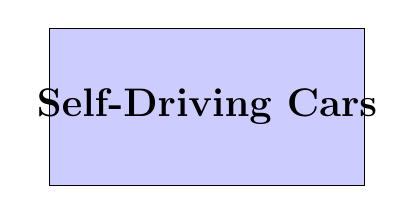
\begin{tikzpicture}[scale=1.2]
			\node[rectangle, draw, fill=blue!20, minimum width=4cm, minimum height=2cm] (car) at (0,0) {};
			\node at (0,0) {\textbf{\Large Self-Driving Cars}};
		\end{tikzpicture}
		\end{center}
	\end{frame}
	
	\begin{frame}{Medical Imaging}
		\begin{center}
		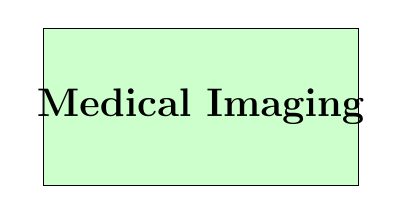
\begin{tikzpicture}[scale=1.2]
			\node[rectangle, draw, fill=green!20, minimum width=4cm, minimum height=2cm] (medical) at (0,0) {};
			\node at (0,0) {\textbf{\Large Medical Imaging}};
		\end{tikzpicture}
		\end{center}
	\end{frame}
	
	\begin{frame}{Smart Retail}
		\begin{center}
		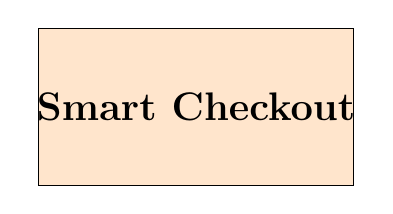
\begin{tikzpicture}[scale=1.2]
			\node[rectangle, draw, fill=orange!20, minimum width=4cm, minimum height=2cm] (retail) at (0,0) {};
			\node at (0,0) {\textbf{\Large Smart Checkout}};
		\end{tikzpicture}
		\end{center}
	\end{frame}
	
	\begin{frame}{Satellite Analysis}
		\begin{center}
		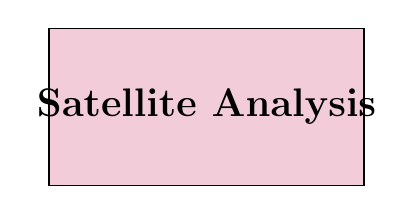
\begin{tikzpicture}[scale=1.2]
			\node[rectangle, draw, fill=purple!20, minimum width=4cm, minimum height=2cm] (satellite) at (0,0) {};
			\node at (0,0) {\textbf{\Large Satellite Analysis}};
		\end{tikzpicture}
		\end{center}
	\end{frame}
	
	\section{What is Object Detection?}
	
	\begin{frame}{Image Classification}
		\begin{center}
		\Large What is Image Classification?
		\end{center}
	\end{frame}
	
	\begin{frame}{Image Classification Goal}
		\begin{center}
		\Large Identify what object is in the image
		\end{center}
	\end{frame}
	
	\begin{frame}{Image Classification Output}
		\begin{center}
		\Large Single class label
		\end{center}
	\end{frame}
	
	\begin{frame}{Image Classification Question}
		\begin{center}
		\Large "What is this?"
		\end{center}
	\end{frame}
	
	\begin{frame}{Object Detection}
		\begin{center}
		\Large What is Object Detection?
		\end{center}
	\end{frame}
	
	\begin{frame}{Object Detection Goal}
		\begin{center}
		\Large Find all objects and their locations
		\end{center}
	\end{frame}
	
	\begin{frame}{Object Detection Output}
		\begin{center}
		\Large Class labels + bounding boxes
		\end{center}
	\end{frame}
	
	\begin{frame}{Object Detection Question}
		\begin{center}
		\Large "What and where?"
		\end{center}
	\end{frame}
	
	\begin{frame}{Detection Components}
		\begin{center}
		\Large What does detection give us?
		\end{center}
	\end{frame}
	
	\begin{frame}{Component 1: Bounding Box}
		\begin{center}
		\Large $(x_{min}, y_{min}, x_{max}, y_{max})$
		\end{center}
	\end{frame}
	
	\begin{frame}{Component 2: Class Label}
		\begin{center}
		\Large Dog, Cat, Car, Person
		\end{center}
	\end{frame}
	
	\begin{frame}{Component 3: Confidence Score}
		\begin{center}
		\Large 0.0 to 1.0
		\end{center}
	\end{frame}
	
	\begin{frame}{Detection Example}
		\begin{center}
		\Large Real detection output
		\end{center}
	\end{frame}
	
	\begin{frame}{Class: Dog}
		\begin{center}
		\Large Class: Dog
		\end{center}
	\end{frame}
	
	\begin{frame}{Confidence: 0.87}
		\begin{center}
		\Large Confidence: 87\%
		\end{center}
	\end{frame}
	
	\begin{frame}{Bounding Box}
		\begin{center}
		\Large (120, 80, 340, 220) pixels
		\end{center}
	\end{frame}
	
	\section{Our 3-Class Detection Example}
	
	\begin{frame}{3-Class Detection}
		\begin{center}
		\Large 3-Class Detection Problem
		\end{center}
	\end{frame}
	
	\begin{frame}{Class 1: Dog}
		\begin{center}
		\Large Dog
		\end{center}
	\end{frame}
	
	\begin{frame}{Class 2: Bicycle}
		\begin{center}
		\Large Bicycle
		\end{center}
	\end{frame}
	
	\begin{frame}{Class 3: Person}
		\begin{center}
		\Large Person
		\end{center}
	\end{frame}
	
	\section{Detection Pipeline}
	
	\begin{frame}{Detection Pipeline}
		\begin{center}
		\Large Object Detection Pipeline
		\end{center}
	\end{frame}
	
	\begin{frame}{Pipeline Input}
		\begin{center}
		\Large Single image with unknown objects
		\end{center}
	\end{frame}
	
	\begin{frame}{Pipeline Processing}
		\begin{center}
		\Large Computer vision algorithms
		\end{center}
	\end{frame}
	
	\begin{frame}{Pipeline Output}
		\begin{center}
		\Large List of detected objects + locations
		\end{center}
	\end{frame}
	
	\begin{frame}{Step 1: Feature Extraction}
		\begin{center}
		\Large Feature Extraction
		\end{center}
	\end{frame}
	
	\begin{frame}{Input Image}
		\begin{center}
		\Large 416×416×3 pixels
		\end{center}
	\end{frame}
	
	\begin{frame}{Backbone Network}
		\begin{center}
		\Large ResNet, EfficientNet, DarkNet
		\end{center}
	\end{frame}
	
	\begin{frame}{Feature Maps}
		\begin{center}
		\Large Rich representations
		\end{center}
	\end{frame}
	
	\begin{frame}{Step 2: Detection Predictions}
		\begin{center}
		\Large Detection Predictions
		\end{center}
	\end{frame}
	
	\begin{frame}{Detection Head}
		\begin{center}
		\Large YOLO, R-CNN, DETR
		\end{center}
	\end{frame}
	
	\begin{frame}{Raw Predictions}
		\begin{center}
		\Large Bounding boxes + class scores
		\end{center}
	\end{frame}
	
	\begin{frame}{Step 3: Post-Processing}
		\begin{center}
		\Large Post-Processing
		\end{center}
	\end{frame}
	
	\begin{frame}{Raw Predictions}
		\begin{center}
		\Large Thousands of boxes
		\end{center}
	\end{frame}
	
	\begin{frame}{NMS + Filtering}
		\begin{center}
		\Large Remove duplicates
		\end{center}
	\end{frame}
	
	\begin{frame}{Final Detections}
		\begin{center}
		\Large Clean results
		\end{center}
	\end{frame}
	
	\section{Evaluation Metrics: The Foundation}
	
	\begin{frame}{Understanding Detection Outcomes}
		\begin{center}
		\begin{tikzpicture}[scale=1.2]
			% Sample image
			\draw[thick] (0,0) rectangle (8,5);
			\node at (4,5.4) {\textbf{Sample Detection Results}};
			
			% True Positive - centered and clear
			\draw[green, very thick] (2,2.5) rectangle (4,4);
			\fill[blue!30] (3,3.25) circle (0.4);
			\node at (3,3.25) {🐶};
			\node[green, font=\large] at (3,2) {\textbf{True Positive (TP)}};
			\node[green] at (3,1.6) {Correctly detected dog};
		\end{tikzpicture}
		\end{center}
		
		\vspace{0.5cm}
		\begin{definitionbox}{True Positive (TP)}
		\textbf{What it means}: The model correctly detected an object that actually exists
		
		\textbf{Requirements}: 
		\begin{itemize}
			\item Object is actually present in ground truth
			\item Model detected it with IoU ≥ threshold (usually 0.5)
		\end{itemize}
		\end{definitionbox}
	\end{frame}
	
	\begin{frame}{False Positive: When Models Hallucinate}
		\begin{center}
		\begin{tikzpicture}[scale=1.2]
			% Sample image
			\draw[thick] (0,0) rectangle (8,5);
			\node at (4,5.4) {\textbf{False Positive Example}};
			
			% False Positive - clear and centered
			\draw[red, very thick] (2.5,2.5) rectangle (4.5,4);
			\node[red, font=\Large] at (3.5,3.25) {❓};
			\node[red, font=\large] at (3.5,2) {\textbf{False Positive (FP)}};
			\node[red] at (3.5,1.6) {Model thinks there's a dog here};
			\node[red] at (3.5,1.3) {but there isn't!};
		\end{tikzpicture}
		\end{center}
		
		\vspace{0.5cm}
		\begin{alertbox}{False Positive (FP)}
		\textbf{What it means}: The model detected an object that doesn't actually exist
		
		\textbf{Common causes}: 
		\begin{itemize}
			\item Confusing background patterns
			\item Low-quality training data
			\item Model overconfidence
		\end{itemize}
		\end{alertbox}
	\end{frame}
	
	\begin{frame}{False Negative: When Models Miss Objects}
		\begin{center}
		\begin{tikzpicture}[scale=1.2]
			% Sample image
			\draw[thick] (0,0) rectangle (8,5);
			\node at (4,5.4) {\textbf{False Negative Example}};
			
			% False Negative - dashed box shows it should be detected
			\draw[orange, very thick, dashed] (2.5,2.5) rectangle (4.5,4);
			\fill[orange!30] (3.5,3.25) circle (0.4);
			\node at (3.5,3.25) {👨‍🦱};
			\node[orange, font=\large] at (3.5,2) {\textbf{False Negative (FN)}};
			\node[orange] at (3.5,1.6) {Person exists but model missed it};
		\end{tikzpicture}
		\end{center}
		
		\vspace{0.5cm}
		\begin{alertbox}{False Negative (FN)}
		\textbf{What it means}: A real object exists but the model failed to detect it
		
		\textbf{Common causes}: 
		\begin{itemize}
			\item Object is partially occluded
			\item Unusual pose or angle
			\item Confidence threshold too high
		\end{itemize}
		\end{alertbox}
	\end{frame}
	
	\begin{frame}{What is Precision?}
		\begin{center}
		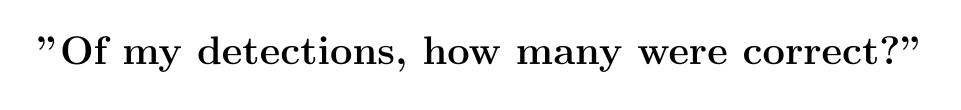
\begin{tikzpicture}[scale=1.5]
			\node[font=\Large] at (0,1) {\textbf{"Of my detections, how many were correct?"}};
		\end{tikzpicture}
		\end{center}
	\end{frame}
	
	\begin{frame}{Precision Formula}
		\begin{center}
		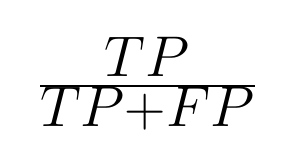
\begin{tikzpicture}[scale=1.5]
			\node[font=\Huge] at (0,1) {$\frac{\text{TP}}{\text{TP + FP}}$};
		\end{tikzpicture}
		\end{center}
	\end{frame}
	
	\begin{frame}{Precision Meaning}
		\begin{center}
		
\begin{tikzpicture}[scale=1.5]
			\node[font=\Large] at (0,1) {\textbf{Correct ÷ All detections}};
		\end{tikzpicture}
		\end{center}
	\end{frame}
	
	\begin{frame}{What is Recall?}
		\begin{center}
		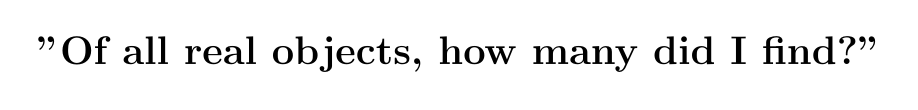
\begin{tikzpicture}[scale=1.5]
			\node[font=\Large] at (0,1) {\textbf{"Of all real objects, how many did I find?"}};
		\end{tikzpicture}
		\end{center}
	\end{frame}
	
	\begin{frame}{Recall Formula}
		\begin{center}
		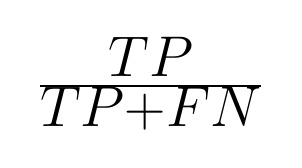
\begin{tikzpicture}[scale=1.5]
			\node[font=\Huge] at (0,1) {$\frac{\text{TP}}{\text{TP + FN}}$};
		\end{tikzpicture}
		\end{center}
	\end{frame}
	
	\begin{frame}{Recall Meaning}
		\begin{center}
		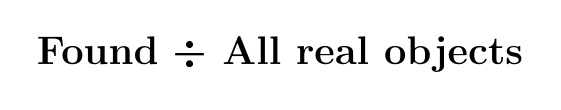
\begin{tikzpicture}[scale=1.5]
			\node[font=\Large] at (0,1) {\textbf{Found ÷ All real objects}};
		\end{tikzpicture}
		\end{center}
	\end{frame}
	
	\begin{frame}{What is IoU?}
		\begin{center}
		
\begin{tikzpicture}[scale=1.5]
			\node[font=\Huge] at (0,1) {\textbf{IoU}};
		\end{tikzpicture}
		\end{center}
	\end{frame}
	
	\begin{frame}{IoU Stands For}
		\begin{center}
		
\begin{tikzpicture}[scale=1.5]
			\node[font=\Large] at (0,1) {\textbf{Intersection over Union}};
		\end{tikzpicture}
		\end{center}
	\end{frame}
	
	\begin{frame}{What Does IoU Measure?}
		\begin{center}
		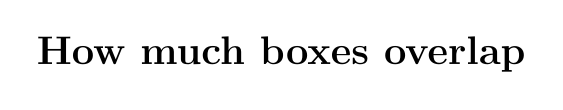
\begin{tikzpicture}[scale=1.5]
			\node[font=\Large] at (0,1) {\textbf{How much boxes overlap}};
		\end{tikzpicture}
		\end{center}
	\end{frame}
	
	\begin{frame}{IoU Range}
		\begin{center}
		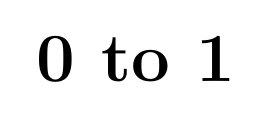
\begin{tikzpicture}[scale=1.5]
			\node[font=\Huge] at (0,1) {\textbf{0 to 1}};
		\end{tikzpicture}
		\end{center}
	\end{frame}
	
	\begin{frame}{Example Setup}
		\begin{center}
		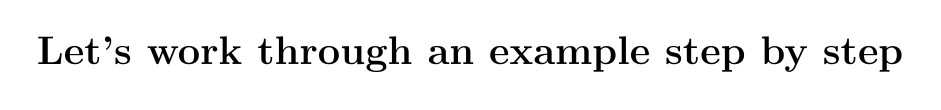
\begin{tikzpicture}[scale=1.5]
			\node[font=\Large] at (0,1) {\textbf{Let's work through an example step by step}};
		\end{tikzpicture}
		\end{center}
	\end{frame}
	
	\begin{frame}{Ground Truth Box}
		\begin{center}
		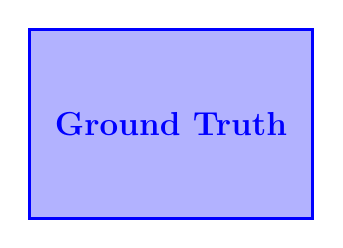
\begin{tikzpicture}[scale=1.2]
			\fill[blue!30] (1,1) rectangle (4,3);
			\draw[blue, very thick] (1,1) rectangle (4,3);
			\node[blue, font=\large] at (2.5,2) {\textbf{Ground Truth}};
		\end{tikzpicture}
		\end{center}
		
		\vspace{1cm}
		\begin{definitionbox}{Coordinates}
		Ground Truth: (1,1) to (4,3)
		\end{definitionbox}
	\end{frame}
	
	\begin{frame}{Prediction Box}
		\begin{center}
		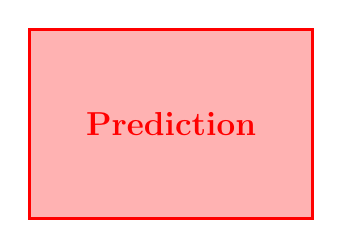
\begin{tikzpicture}[scale=1.2]
			\fill[red!30] (2,0.5) rectangle (5,2.5);
			\draw[red, very thick] (2,0.5) rectangle (5,2.5);
			\node[red, font=\large] at (3.5,1.5) {\textbf{Prediction}};
		\end{tikzpicture}
		\end{center}
		
		\vspace{1cm}
		\begin{definitionbox}{Coordinates}
		Prediction: (2,0.5) to (5,2.5)
		\end{definitionbox}
	\end{frame}
	
	\begin{frame}{Both Boxes Together}
		\begin{center}
		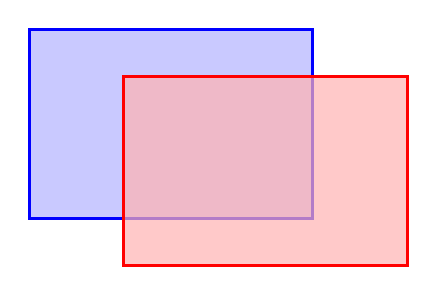
\begin{tikzpicture}[scale=1.2]
			% Ground truth
			\fill[blue!30, opacity=0.7] (1,1) rectangle (4,3);
			\draw[blue, very thick] (1,1) rectangle (4,3);
			
			% Prediction
			\fill[red!30, opacity=0.7] (2,0.5) rectangle (5,2.5);
			\draw[red, very thick] (2,0.5) rectangle (5,2.5);
		\end{tikzpicture}
		\end{center}
		
		\vspace{1cm}
		\begin{definitionbox}{Question}
		Where do they overlap?
		\end{definitionbox}
	\end{frame}
	
	\begin{frame}{Finding Intersection - X Coordinates}
		\begin{center}
		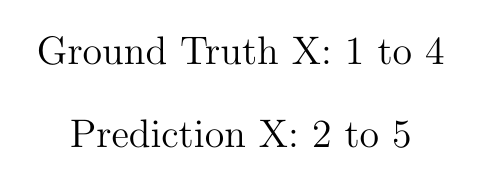
\begin{tikzpicture}[scale=1.5]
			\node[font=\Large] at (0,1) {Ground Truth X: 1 to 4};
			\node[font=\Large] at (0,0.3) {Prediction X: 2 to 5};
		\end{tikzpicture}
		\end{center}
		
		\vspace{1cm}
		\begin{examplebox}{Step 1}
		Overlap X: from max(1,2) = 2 to min(4,5) = 4
		\end{examplebox}
	\end{frame}
	
	\begin{frame}{Finding Intersection - Y Coordinates}
		\begin{center}
		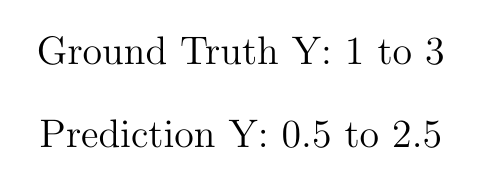
\begin{tikzpicture}[scale=1.5]
			\node[font=\Large] at (0,1) {Ground Truth Y: 1 to 3};
			\node[font=\Large] at (0,0.3) {Prediction Y: 0.5 to 2.5};
		\end{tikzpicture}
		\end{center}
		
		\vspace{1cm}
		\begin{examplebox}{Step 2}
		Overlap Y: from max(1,0.5) = 1 to min(3,2.5) = 2.5
		\end{examplebox}
	\end{frame}
	
	\begin{frame}{Intersection Rectangle}
		\begin{center}
		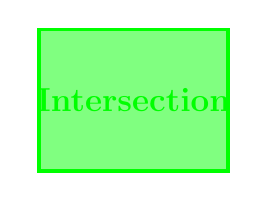
\begin{tikzpicture}[scale=1.2]
			% Show intersection only
			\fill[green!50] (2,1) rectangle (4,2.5);
			\draw[green, very thick] (2,1) rectangle (4,2.5);
			\node[green, font=\large] at (3,1.75) {\textbf{Intersection}};
		\end{tikzpicture}
		\end{center}
		
		\vspace{1cm}
		\begin{definitionbox}{Intersection Box}
		From (2,1) to (4,2.5)
		\end{definitionbox}
	\end{frame}
	
	\begin{frame}{Calculate Intersection Width}
		\begin{center}
		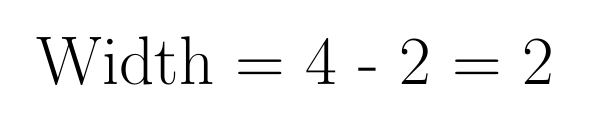
\begin{tikzpicture}[scale=1.5]
			\node[font=\Huge] at (0,1) {Width = 4 - 2 = 2};
		\end{tikzpicture}
		\end{center}
		
		\vspace{1cm}
		\begin{examplebox}{Step 3}
		Right edge - Left edge = Width
		\end{examplebox}
	\end{frame}
	
	\begin{frame}{Calculate Intersection Height}
		\begin{center}
		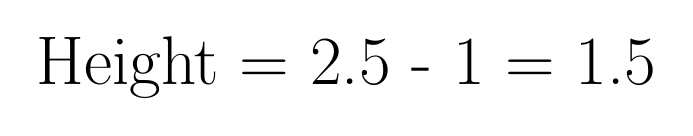
\begin{tikzpicture}[scale=1.5]
			\node[font=\Huge] at (0,1) {Height = 2.5 - 1 = 1.5};
		\end{tikzpicture}
		\end{center}
		
		\vspace{1cm}
		\begin{examplebox}{Step 4}
		Top edge - Bottom edge = Height
		\end{examplebox}
	\end{frame}
	
	\begin{frame}{Calculate Intersection Area}
		\begin{center}
		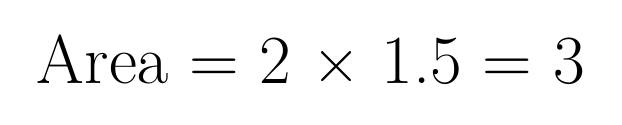
\begin{tikzpicture}[scale=1.5]
			\node[font=\Huge] at (0,1) {Area = 2 × 1.5 = 3};
		\end{tikzpicture}
		\end{center}
		
		\vspace{1cm}
		\begin{definitionbox}{Step 5}
		Width × Height = Area
		\end{definitionbox}
	\end{frame}
	
	\begin{frame}{IoU: Calculating the Union}
		\begin{center}
		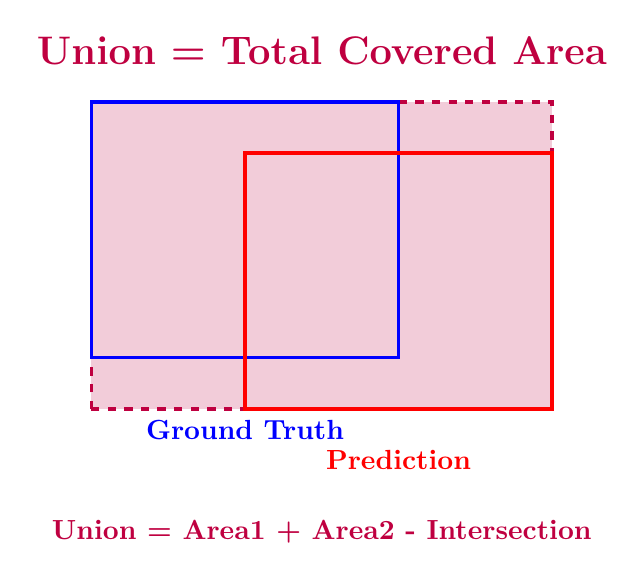
\begin{tikzpicture}[scale=1.3]
			% Union area (everything covered by either box)
			\fill[purple!20] (1,1.5) rectangle (5.5,4.5);
			\draw[purple, very thick, dashed] (1,1.5) rectangle (5.5,4.5);
			\node[purple, font=\Large] at (3.25,5) {\textbf{Union = Total Covered Area}};
			
			% Ground truth box
			\draw[blue, very thick] (1,2) rectangle (4,4.5);
			\node[blue] at (2.5,1.3) {\textbf{Ground Truth}};
			
			% Predicted box
			\draw[red, very thick] (2.5,1.5) rectangle (5.5,4);
			\node[red] at (4,1) {\textbf{Prediction}};
			
			% Show the formula visually
			\node[purple] at (3.25,0.3) {\textbf{Union = Area1 + Area2 - Intersection}};
		\end{tikzpicture}
		\end{center}
		
	\end{frame}
	
	\begin{frame}{Now Calculate Union}
		\begin{center}
		
\begin{tikzpicture}[scale=1.5]
			\node[font=\Large] at (0,1) {\textbf{Union = Area1 + Area2 - Intersection}};
		\end{tikzpicture}
		\end{center}
		
		\vspace{1cm}
		\begin{definitionbox}{Why Subtract?}
		We subtract intersection to avoid counting it twice
		\end{definitionbox}
	\end{frame}
	
	\begin{frame}{Ground Truth Area}
		\begin{center}
		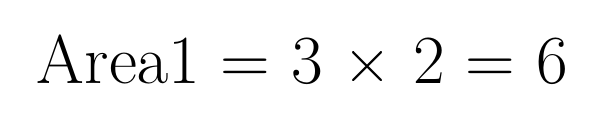
\begin{tikzpicture}[scale=1.5]
			\node[font=\Huge] at (0,1) {Area1 = 3 × 2 = 6};
		\end{tikzpicture}
		\end{center}
		
		\vspace{1cm}
		\begin{examplebox}{Step 6}
		Ground Truth: Width 3, Height 2
		\end{examplebox}
	\end{frame}
	
	\begin{frame}{Prediction Area}
		\begin{center}
		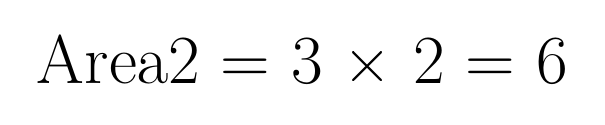
\begin{tikzpicture}[scale=1.5]
			\node[font=\Huge] at (0,1) {Area2 = 3 × 2 = 6};
		\end{tikzpicture}
		\end{center}
		
		\vspace{1cm}
		\begin{examplebox}{Step 7}
		Prediction: Width 3, Height 2
		\end{examplebox}
	\end{frame}
	
	\begin{frame}{Calculate Union}
		\begin{center}
		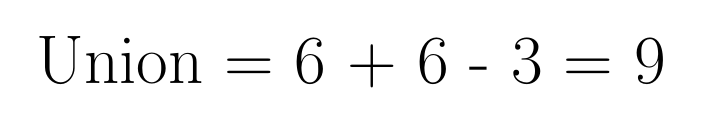
\begin{tikzpicture}[scale=1.5]
			\node[font=\Huge] at (0,1) {Union = 6 + 6 - 3 = 9};
		\end{tikzpicture}
		\end{center}
		
		\vspace{1cm}
		\begin{definitionbox}{Step 8}
		Area1 + Area2 - Intersection = Union
		\end{definitionbox}
	\end{frame}
	
	\begin{frame}{IoU: The Formula}
		\begin{center}
		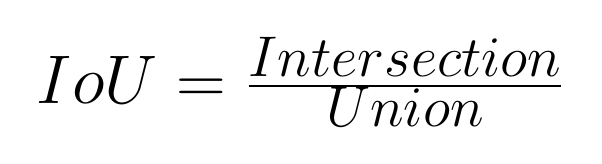
\begin{tikzpicture}[scale=1.5]
			\node[font=\Huge] at (0,2) {$\text{IoU} = \frac{\text{Intersection}}{\text{Union}}$};
		\end{tikzpicture}
		\end{center}
		
		\vspace{1cm}
		\begin{definitionbox}{Simple Division}
		Take the overlapping area and divide by the total covered area
		\end{definitionbox}
	\end{frame}
	
	\begin{frame}{Final IoU Calculation}
		\begin{center}
		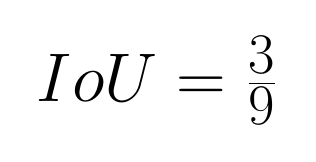
\begin{tikzpicture}[scale=1.5]
			\node[font=\Huge] at (0,1) {$\text{IoU} = \frac{3}{9}$};
		\end{tikzpicture}
		\end{center}
		
		\vspace{1cm}
		\begin{examplebox}{Step 9}
		Intersection ÷ Union
		\end{examplebox}
	\end{frame}
	
	\begin{frame}{Do the Division}
		\begin{center}
		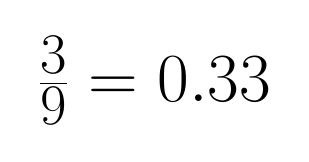
\begin{tikzpicture}[scale=1.5]
			\node[font=\Huge] at (0,1) {$\frac{3}{9} = 0.33$};
		\end{tikzpicture}
		\end{center}
		
		\vspace{1cm}
		\begin{definitionbox}{Final Answer}
		IoU = 0.33 (33% overlap)
		\end{definitionbox}
	\end{frame}
	
	\begin{frame}{IoU Threshold: 0.5}
		\begin{center}
		\begin{tikzpicture}[scale=1.5]
			\node[font=\Huge] at (0,1) {IoU ≥ 0.5};
		\end{tikzpicture}
		\end{center}
		
		\vspace{1cm}
		\begin{definitionbox}{Standard Rule}
		If IoU is 0.5 or higher, we call it a True Positive
		\end{definitionbox}
	\end{frame}
	
	\begin{frame}{IoU Below Threshold}
		\begin{center}
		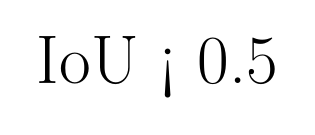
\begin{tikzpicture}[scale=1.5]
			\node[font=\Huge] at (0,1) {IoU < 0.5};
		\end{tikzpicture}
		\end{center}
		
		\vspace{1cm}
		\begin{alertbox}{False Positive}
		If IoU is below 0.5, we call it a False Positive
		\end{alertbox}
	\end{frame}
	
	\stepcounter{popquiz}
	\begin{frame}{Pop Quiz \#\thepopquiz}
		\begin{popquizbox}{\thepopquiz}
		Given this detection scenario:
		\begin{itemize}
			\item Ground Truth: 5 dogs in image
			\item Model detections: 8 boxes predicted as "dog"
			\item 4 detections have IoU ≥ 0.5 with ground truth
		\end{itemize}
		
		What are TP, FP, FN, Precision, and Recall?
		
		\begin{enumerate}[A)]
			\item TP=4, FP=4, FN=1, Precision=0.5, Recall=0.8
			\item TP=5, FP=3, FN=0, Precision=0.63, Recall=1.0
			\item TP=4, FP=1, FN=4, Precision=0.8, Recall=0.5
			\item TP=8, FP=0, FN=0, Precision=1.0, Recall=1.0
		\end{enumerate}
		\end{popquizbox}
	\end{frame}
	
	\begin{frame}{The Answer}
		\begin{center}
		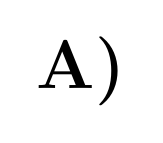
\begin{tikzpicture}[scale=1.5]
			\node[font=\Huge] at (0,1) {\textbf{A)}} ;
		\end{tikzpicture}
		\end{center}
		
		\vspace{1cm}
		\begin{definitionbox}{Correct Answer}
		TP=4, FP=4, FN=1, Precision=0.5, Recall=0.8
		\end{definitionbox}
	\end{frame}
	
	\begin{frame}{Step 1: Find TP}
		\begin{center}
		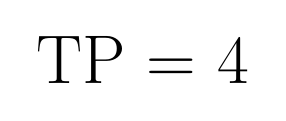
\begin{tikzpicture}[scale=1.5]
			\node[font=\Huge] at (0,1) {TP = 4};
		\end{tikzpicture}
		\end{center}
		
		\vspace{1cm}
		\begin{examplebox}{Explanation}
		4 detections have IoU ≥ 0.5 with ground truth
		\end{examplebox}
	\end{frame}
	
	\begin{frame}{Step 2: Find FP}
		\begin{center}
		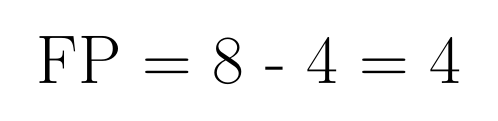
\begin{tikzpicture}[scale=1.5]
			\node[font=\Huge] at (0,1) {FP = 8 - 4 = 4};
		\end{tikzpicture}
		\end{center}
		
		\vspace{1cm}
		\begin{examplebox}{Explanation}
		8 total detections - 4 correct = 4 false alarms
		\end{examplebox}
	\end{frame}
	
	\begin{frame}{Step 3: Find FN}
		\begin{center}
		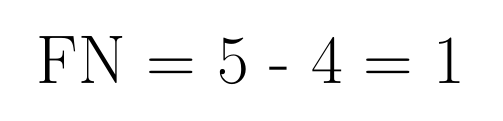
\begin{tikzpicture}[scale=1.5]
			\node[font=\Huge] at (0,1) {FN = 5 - 4 = 1};
		\end{tikzpicture}
		\end{center}
		
		\vspace{1cm}
		\begin{examplebox}{Explanation}
		5 ground truth dogs - 4 detected = 1 missed
		\end{examplebox}
	\end{frame}
	
	\begin{frame}{Step 4: Calculate Precision}
		\begin{center}
		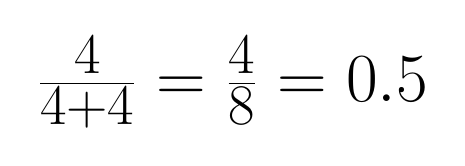
\begin{tikzpicture}[scale=1.5]
			\node[font=\Huge] at (0,1) {$\frac{4}{4+4} = \frac{4}{8} = 0.5$};
		\end{tikzpicture}
		\end{center}
		
		\vspace{1cm}
		\begin{definitionbox}{Precision Formula}
		TP ÷ (TP + FP)
		\end{definitionbox}
	\end{frame}
	
	\begin{frame}{Step 5: Calculate Recall}
		\begin{center}
		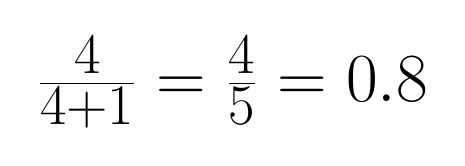
\begin{tikzpicture}[scale=1.5]
			\node[font=\Huge] at (0,1) {$\frac{4}{4+1} = \frac{4}{5} = 0.8$};
		\end{tikzpicture}
		\end{center}
		
		\vspace{1cm}
		\begin{definitionbox}{Recall Formula}
		TP ÷ (TP + FN)
		\end{definitionbox}
	\end{frame}
	
	\section{Precision-Recall Curves and Average Precision}
	
	\begin{frame}{Precision-Recall Curve}
		\begin{columns}
		\begin{column}{0.55\textwidth}
			\begin{center}
			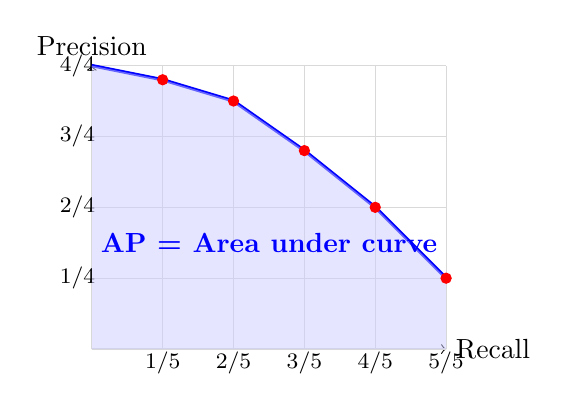
\begin{tikzpicture}[scale=0.9]
				% Axes
				\draw[->] (0,0) -- (5,0) node[right] {Recall};
				\draw[->] (0,0) -- (0,4) node[above] {Precision};
				
				% Grid
				\draw[gray!30] (0,0) grid (5,4);
				
				% Ticks
				\foreach \x in {1,2,3,4,5} \node at (\x,-0.2) {\footnotesize \x/5};
				\foreach \y in {1,2,3,4} \node at (-0.2,\y) {\footnotesize \y/4};
				
				% PR Curve
				\draw[blue, very thick] (0,4) -- (1,3.8) -- (2,3.5) -- (3,2.8) -- (4,2) -- (5,1);
				\fill[blue!20, opacity=0.5] (0,4) -- (1,3.8) -- (2,3.5) -- (3,2.8) -- (4,2) -- (5,1) -- (5,0) -- (0,0) -- cycle;
				
				% Points
				\foreach \x/\y in {1/3.8,2/3.5,3/2.8,4/2,5/1} {
					\fill[red] (\x,\y) circle (0.08);
				}
				
				% Labels
				\node at (2.5,1.5) {\textcolor{blue}{\textbf{AP = Area under curve}}};
			\end{tikzpicture}
			\end{center}
		\end{column}
		
		\begin{column}{0.4\textwidth}
			\begin{definitionbox}{PR Curve Interpretation}
			\begin{itemize}
				\item \textbf{High precision at low recall}: Easy detections first
				\item \textbf{Curve drops}: As we include more detections, precision falls
				\item \textbf{Area Under Curve}: Average Precision (AP)
			\end{itemize}
			\end{definitionbox}
		\end{column}
		\end{columns}
		
		\vspace{0.3cm}
		\begin{examplebox}{Average Precision (AP)}
		$$\text{AP} = \int_0^1 \text{Precision}(r) \, dr$$
		\textbf{Intuition}: A perfect detector has AP = 1.0, while a random detector has AP ≈ 0.5
		\end{examplebox}
	\end{frame}
	
	\begin{frame}{Computing AP: Step-by-Step Example}
		\begin{center}
		\begin{examplebox}{Dog Detection Results (Sorted by Confidence)}
		\begin{tabular}{|c|c|c|c|c|c|}
		\hline
		\textbf{Detection} & \textbf{Confidence} & \textbf{IoU} & \textbf{TP/FP} & \textbf{Precision} & \textbf{Recall} \\
		\hline
		1 & 0.95 & 0.8 & TP & 1/1 = 1.00 & 1/3 = 0.33 \\
		2 & 0.89 & 0.3 & FP & 1/2 = 0.50 & 1/3 = 0.33 \\
		3 & 0.76 & 0.7 & TP & 2/3 = 0.67 & 2/3 = 0.67 \\
		4 & 0.65 & 0.6 & TP & 3/4 = 0.75 & 3/3 = 1.00 \\
		5 & 0.43 & 0.2 & FP & 3/5 = 0.60 & 3/3 = 1.00 \\
		\hline
		\end{tabular}
		\end{examplebox}
		\end{center}
		
		\begin{keypointsbox}
		\textbf{Ground Truth}: 3 dogs in image \\
		\textbf{AP Calculation} (using trapezoidal rule):
		\begin{align}
		\text{AP} &= \frac{1}{2}[(1.00 + 0.67) \times 0.34 + (0.67 + 0.75) \times 0.33 + (0.75 + 0.60) \times 0.00] \\
		&= \frac{1}{2}[0.57 + 0.47 + 0] = 0.52
		\end{align}
		\end{keypointsbox}
	\end{frame}
	
	\section{Mean Average Precision (mAP)}
	
	\begin{frame}{From AP to mAP: Multi-Class Evaluation}
		\begin{center}
		\begin{examplebox}{3-Class Example: Computing Individual APs}
		\begin{tabular}{|c|c|c|}
		\hline
		\textbf{Class} & \textbf{Ground Truth Count} & \textbf{Average Precision (AP)} \\
		\hline
		🐶 Dog & 12 objects & AP = 0.73 \\
		🚲 Bicycle & 8 objects & AP = 0.65 \\
		👨‍🦱 Person & 15 objects & AP = 0.81 \\
		\hline
		\end{tabular}
		\end{examplebox}
		\end{center}
		
		\begin{definitionbox}{Mean Average Precision (mAP)}
		$$\text{mAP} = \frac{1}{C} \sum_{c=1}^{C} \text{AP}_c$$
		
		\textbf{For our example:}
		$$\text{mAP} = \frac{1}{3}(0.73 + 0.65 + 0.81) = \frac{2.19}{3} = 0.73$$
		\end{definitionbox}
		
		\begin{keypointsbox}
		\textbf{mAP Interpretation:}
		\begin{itemize}
			\item \textbf{0.73}: Good performance across all classes
			\item \textbf{Balanced}: No single class dominates the metric
			\item \textbf{Standard}: Most papers report mAP for model comparison
		\end{itemize}
		\end{keypointsbox}
	\end{frame}
	
	\begin{frame}{mAP Variants: @50, @75, @[.5:.95]}
		\begin{center}
		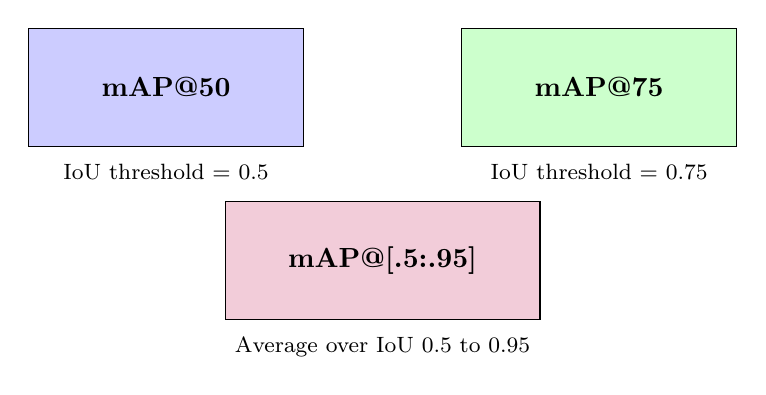
\begin{tikzpicture}[scale=1.1]
			% mAP@50
			\node[rectangle, draw, fill=blue!20, minimum width=3.5cm, minimum height=1.5cm] (map50) at (0,2) {};
			\node at (0,2) {\textbf{mAP@50}};
			\node[below=0.1cm of map50] {\footnotesize IoU threshold = 0.5};
			
			% mAP@75
			\node[rectangle, draw, fill=green!20, minimum width=3.5cm, minimum height=1.5cm] (map75) at (5,2) {};
			\node at (5,2) {\textbf{mAP@75}};
			\node[below=0.1cm of map75] {\footnotesize IoU threshold = 0.75};
			
			% mAP@[.5:.95]
			\node[rectangle, draw, fill=purple!20, minimum width=4cm, minimum height=1.5cm] (maprange) at (2.5,0) {};
			\node at (2.5,0) {\textbf{mAP@[.5:.95]}};
			\node[below=0.1cm of maprange] {\footnotesize Average over IoU 0.5 to 0.95};
		\end{tikzpicture}
		\end{center}
		
		\begin{examplebox}{Example Results Comparison}
		\begin{tabular}{|c|c|c|}
		\hline
		\textbf{Metric} & \textbf{Value} & \textbf{Interpretation} \\
		\hline
		mAP@50 & 0.73 & Good localization (loose) \\
		mAP@75 & 0.52 & Moderate localization (strict) \\
		mAP@[.5:.95] & 0.61 & COCO-style evaluation \\
		\hline
		\end{tabular}
		\end{examplebox}
		
		\begin{alertbox}{Key Insight}
		\textbf{mAP@75 < mAP@50}: Stricter IoU threshold = lower scores. COCO benchmark uses mAP@[.5:.95] as the primary metric!
		\end{alertbox}
	\end{frame}
	
	\section{Advanced Topics}
	
	\begin{frame}{Class-Agnostic mAP}
		\begin{definitionbox}{What is Class-Agnostic Detection?}
		Instead of predicting specific classes, we just ask: \textbf{"Is there any object here?"}
		\end{definitionbox}
		
		\begin{center}
		\begin{tikzpicture}[scale=0.9]
			% Regular detection
			\node at (2,4) {\textbf{Regular Detection}};
			\draw[thick] (0,2.5) rectangle (4,3.5);
			\draw[red, thick] (0.5,2.7) rectangle (1.5,3.3);
			\node at (1,3) {🐶};
			\node[red] at (1,2.5) {\footnotesize Dog: 0.87};
			
			\draw[blue, thick] (2.5,2.7) rectangle (3.5,3.3);
			\node at (3,3) {🚲};
			\node[blue] at (3,2.5) {\footnotesize Bike: 0.92};
			
			% Class-agnostic
			\node at (2,1.5) {\textbf{Class-Agnostic Detection}};
			\draw[thick] (0,0) rectangle (4,1);
			\draw[green, thick] (0.5,0.2) rectangle (1.5,0.8);
			\node at (1,0.5) {🐶};
			\node[green] at (1,0) {\footnotesize Object: 0.87};
			
			\draw[green, thick] (2.5,0.2) rectangle (3.5,0.8);
			\node at (3,0.5) {🚲};
			\node[green] at (3,0) {\footnotesize Object: 0.92};
		\end{tikzpicture}
		\end{center}
		
		\begin{examplebox}{Use Cases for Class-Agnostic mAP}
		\begin{itemize}
			\item \textbf{Weak supervision}: When you don't have class labels
			\item \textbf{General objectness}: Focus on localization, not classification
			\item \textbf{Domain adaptation}: Transfer detection across domains
		\end{itemize}
		\end{examplebox}
	\end{frame}
	
	\begin{frame}{Negative Set Evaluation}
		\begin{alertbox}{Challenge: What about images with NO objects?}
		\end{alertbox}
		
		\begin{center}
		\begin{tikzpicture}[scale=1.1]
			% Negative image
			\draw[thick] (0,0) rectangle (4,3);
			\node at (2,3.3) {\textbf{Negative Image (No Objects)}};
			
			% Landscape elements
			\fill[green!30] (0,0) rectangle (4,1);
			\fill[blue!30] (0,1) rectangle (4,1.5);
			\fill[yellow!30] (1,1.5) circle (0.3);
			\node at (2,0.5) {🌳🌲🌳};
			
			% False positive detection
			\draw[red, very thick] (2.5,1.8) rectangle (3.5,2.5);
			\node[red] at (3,2.65) {\footnotesize FP: Dog 0.63};
			
			% Stats
			\node[align=left] at (6,1.5) {
				\textbf{Results:} \\
				TP = 0 (no ground truth) \\
				FP = 1 (false detection) \\
				FN = 0 (no ground truth) \\[0.3cm]
				Precision = $\frac{0}{0+1} = 0$ \\
				Recall = undefined
			};
		\end{tikzpicture}
		\end{center}
		
		\begin{keypointsbox}
		\textbf{Negative Set Metrics:}
		\begin{itemize}
			\item \textbf{False Positive Rate}: FP detections per negative image
			\item \textbf{Precision = 0} if any FP detections exist
			\item Important for real-world deployment!
		\end{itemize}
		\end{keypointsbox}
	\end{frame}
	
	\section{Common Detection Errors}
	
	\begin{frame}{Localization vs Classification Errors}
		\begin{center}
		\begin{tikzpicture}[scale=0.9]
			% Ground truth
			\node at (2,5.2) {\textbf{Ground Truth}};
			\draw[thick] (0,3.5) rectangle (4,4.8);
			\draw[blue, thick] (1,3.8) rectangle (2,4.5);
			\node at (1.5,4.15) {🐶};
			\node[blue] at (1.5,3.4) {\footnotesize Dog};
			
			% Localization error
			\node at (2,2.5) {\textbf{Localization Error}};
			\draw[thick] (0,0.8) rectangle (4,2.1);
			\draw[red, thick] (2.2,1.1) rectangle (3.2,1.8);
			\node at (1.5,1.45) {🐶};
			\node[red] at (2.7,0.5) {\footnotesize Dog (IoU=0.3)};
			
			% Class error
			\node at (7.5,5.2) {\textbf{Classification Error}};
			\draw[thick] (5.5,3.5) rectangle (9.5,4.8);
			\draw[orange, thick] (6.5,3.8) rectangle (7.5,4.5);
			\node at (7,4.15) {🐶};
			\node[orange] at (7,3.4) {\footnotesize Cat (IoU=0.8)};
			
			% Duplicate detection
			\node at (7.5,2.5) {\textbf{Duplicate Detection}};
			\draw[thick] (5.5,0.8) rectangle (9.5,2.1);
			\draw[green, thick] (6.3,1.1) rectangle (7.3,1.8);
			\draw[purple, thick] (6.8,1.0) rectangle (7.8,1.7);
			\node at (7,1.45) {🐶};
			\node[green] at (6.8,0.5) {\footnotesize Dog 0.9};
			\node[purple] at (7.8,0.5) {\footnotesize Dog 0.7};
		\end{tikzpicture}
		\end{center}
		
		\begin{definitionbox}{Error Types}
		\begin{itemize}
			\item \textbf{Localization Error}: Right class, wrong location (IoU < threshold)
			\item \textbf{Classification Error}: Right location, wrong class
			\item \textbf{Duplicate Detection}: Multiple boxes for same object
		\end{itemize}
		\end{definitionbox}
	\end{frame}
	
	\stepcounter{popquiz}
	\begin{frame}{Pop Quiz \#\thepopquiz}
		\begin{popquizbox}{\thepopquiz}
		You have a dataset with:
		\begin{itemize}
			\item 100 images total
			\item 50 images with dogs (300 dog instances total)
			\item 50 negative images (no objects)
		\end{itemize}
		
		Your model detects:
		\begin{itemize}
			\item 250 dogs correctly (IoU ≥ 0.5)
			\item 30 false positive dogs in positive images
			\item 20 false positive dogs in negative images
		\end{itemize}
		
		What is the Precision and Recall for the Dog class?
		
		\begin{enumerate}[A)]
			\item Precision=0.83, Recall=0.83
			\item Precision=0.89, Recall=0.75
			\item Precision=0.75, Recall=0.89
		\end{enumerate}
		\end{popquizbox}
	\end{frame}
	
	\begin{frame}{Pop Quiz \#\thepopquiz{} - Answer}
		\textbf{Answer: A) Precision=0.83, Recall=0.83}
		
		\begin{examplebox}{Step-by-Step Calculation}
		\textbf{Given:}
		\begin{itemize}
			\item TP = 250 (correctly detected dogs)
			\item FP = 30 + 20 = 50 (false positives in positive + negative images)
			\item FN = 300 - 250 = 50 (ground truth dogs - detected dogs)
		\end{itemize}
		
		\textbf{Calculations:}
		\begin{align}
		\text{Precision} &= \frac{\text{TP}}{\text{TP + FP}} = \frac{250}{250 + 50} = \frac{250}{300} = 0.83 \\
		\text{Recall} &= \frac{\text{TP}}{\text{TP + FN}} = \frac{250}{250 + 50} = \frac{250}{300} = 0.83
		\end{align}
		\end{examplebox}
	\end{frame}
	
	\section{Summary and Practical Applications}
	
	\begin{frame}{What is AP?}
		\begin{center}
		
\begin{tikzpicture}[scale=1.5]
			\node[font=\Huge] at (0,1) {\textbf{AP}};
			\node[font=\large] at (0,0.3) {Average Precision};
		\end{tikzpicture}
		\end{center}
		
		\vspace{1cm}
		\begin{definitionbox}{One Class}
		AP measures performance for one single class
		\end{definitionbox}
	\end{frame}
	
	\begin{frame}{What is mAP?}
		\begin{center}
		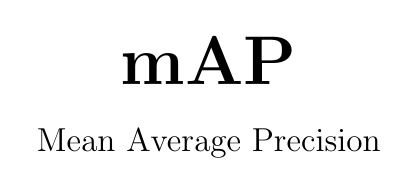
\begin{tikzpicture}[scale=1.5]
			\node[font=\Huge] at (0,1) {\textbf{mAP}};
			\node[font=\large] at (0,0.3) {Mean Average Precision};
		\end{tikzpicture}
		\end{center}
		
		\vspace{1cm}
		\begin{definitionbox}{All Classes}
		mAP is the average of AP across all classes
		\end{definitionbox}
	\end{frame}
	
	\begin{frame}{mAP Example Setup}
		\begin{center}
		\begin{tikzpicture}[scale=1.5]
			\node[font=\Large] at (0,1) {\textbf{Let's calculate mAP for 3 classes}};
		\end{tikzpicture}
		\end{center}
	\end{frame}
	
	\begin{frame}{AP for Dogs}
		\begin{center}
		\begin{tikzpicture}[scale=1.5]
			\node[font=\Huge] at (0,1) {AP\_dogs = 0.8};
		\end{tikzpicture}
		\end{center}
		
		\vspace{1cm}
		\begin{examplebox}{Given}
		Dog class achieved 80% average precision
		\end{examplebox}
	\end{frame}
	
	\begin{frame}{AP for Cats}
		\begin{center}
		\begin{tikzpicture}[scale=1.5]
			\node[font=\Huge] at (0,1) {AP\_cats = 0.6};
		\end{tikzpicture}
		\end{center}
		
		\vspace{1cm}
		\begin{examplebox}{Given}
		Cat class achieved 60% average precision
		\end{examplebox}
	\end{frame}
	
	\begin{frame}{AP for Cars}
		\begin{center}
		\begin{tikzpicture}[scale=1.5]
			\node[font=\Huge] at (0,1) {AP\_cars = 0.9};
		\end{tikzpicture}
		\end{center}
		
		\vspace{1cm}
		\begin{examplebox}{Given}
		Car class achieved 90% average precision
		\end{examplebox}
	\end{frame}
	
	\begin{frame}{Add Them Up}
		\begin{center}
		\begin{tikzpicture}[scale=1.5]
			\node[font=\Huge] at (0,1) {0.8 + 0.6 + 0.9 = 2.3};
		\end{tikzpicture}
		\end{center}
		
		\vspace{1cm}
		\begin{examplebox}{Step 1}
		Sum all the AP values
		\end{examplebox}
	\end{frame}
	
	\begin{frame}{Divide by Number of Classes}
		\begin{center}
		\begin{tikzpicture}[scale=1.5]
			\node[font=\Huge] at (0,1) {$\frac{2.3}{3} = 0.77$};
		\end{tikzpicture}
		\end{center}
		
		\vspace{1cm}
		\begin{definitionbox}{Final Answer}
		mAP = 0.77 (77%)
		\end{definitionbox}
	\end{frame}
	
	\begin{frame}{mAP@50}
		\begin{center}
		\begin{tikzpicture}[scale=1.5]
			\node[font=\Huge] at (0,1) {\textbf{mAP@50}};
		\end{tikzpicture}
		\end{center}
		
		\vspace{1cm}
		\begin{definitionbox}{Standard Evaluation}
		Uses IoU threshold of 0.5
		\end{definitionbox}
	\end{frame}
	
	\begin{frame}{Specialized mAP Variants}
		\begin{center}
		\begin{tikzpicture}[scale=1.1]
			% Class-Agnostic mAP
			\node[rectangle, draw, fill=teal!15, minimum width=6cm, minimum height=2cm, rounded corners=8pt] (camap) at (0,1.5) {};
			\node[teal, font=\Large] at (0,2.2) {\textbf{Class-Agnostic mAP}};
			\node[align=center] at (0,1.5) {Ignores class labels\\Just asks: "Is there an object?"};
			\node[teal, font=\small] at (0,1) {Useful for weakly supervised learning};
			
			% Size-specific mAP
			\node[rectangle, draw, fill=red!15, minimum width=6cm, minimum height=2cm, rounded corners=8pt] (sizemap) at (0,-1.5) {};
			\node[red, font=\Large] at (0,-0.8) {\textbf{Size-Specific mAP}};
			\node[align=center] at (0,-1.5) {Separate evaluation for\\small, medium, large objects};
			\node[red, font=\small] at (0,-2) {COCO provides mAP\_S, mAP\_M, mAP\_L};
		\end{tikzpicture}
		\end{center}
		
	\end{frame}
	
	\begin{frame}{Summary}
		\begin{center}
		\begin{tikzpicture}[scale=1.5]
			\node[font=\Huge] at (0,1) {\textbf{That's It!}};
		\end{tikzpicture}
		\end{center}
		
		\vspace{1cm}
		\begin{definitionbox}{Key Point}
		Object detection uses mAP to measure performance
		\end{definitionbox}
	\end{frame}
	
	\begin{frame}{Detection Fundamentals: Key Takeaways}
		\begin{center}
		\begin{tikzpicture}[scale=0.9]
			% Main equation
			\node[rectangle, draw, fill=yellow!20, minimum width=8cm, minimum height=1.5cm, rounded corners=12pt] (eq) at (0,3) {};
			\node[font=\LARGE] at (0,3) {\textbf{Object Detection = Classification + Localization}};
			
			% Supporting points
			\node[rectangle, draw, fill=blue!10, minimum width=7cm, minimum height=1cm, rounded corners=8pt] (point1) at (0,1.5) {};
			\node at (0,1.5) {\textbf{mAP is the gold standard} for model comparison};
			
			\node[rectangle, draw, fill=green!10, minimum width=7cm, minimum height=1cm, rounded corners=8pt] (point2) at (0,0.3) {};
			\node at (0,0.3) {\textbf{IoU thresholds matter} - stricter = lower scores};
			
			\node[rectangle, draw, fill=red!10, minimum width=7cm, minimum height=1cm, rounded corners=8pt] (point3) at (0,-0.9) {};
			\node at (0,-0.9) {\textbf{Negative images} crucial for real deployment};
			
			\node[rectangle, draw, fill=purple!10, minimum width=7cm, minimum height=1cm, rounded corners=8pt] (point4) at (0,-2.1) {};
			\node at (0,-2.1) {\textbf{Context matters} - choose metrics for your use case};
		\end{tikzpicture}
		\end{center}
		
		\begin{definitionbox}{Remember}
		Perfect metrics don't guarantee perfect real-world performance. Always test in your target domain!
		\end{definitionbox}
	\end{frame}
	
	\begin{frame}{Real-World Considerations}
		\begin{alertbox}{Beyond the Metrics}
		Perfect mAP doesn't guarantee perfect real-world performance!
		\end{alertbox}
		
		\begin{columns}
		\begin{column}{0.48\textwidth}
			\begin{examplebox}{Model Selection}
			\begin{itemize}
				\item \textbf{Speed vs Accuracy}: YOLOv8 vs R-CNN
				\item \textbf{Memory constraints}: Mobile deployment
				\item \textbf{Class imbalance}: Rare vs common objects
			\end{itemize}
			\end{examplebox}
		\end{column}
		
		\begin{column}{0.48\textwidth}
			\begin{definitionbox}{Deployment Issues}
			\begin{itemize}
				\item \textbf{Domain shift}: Training vs real data
				\item \textbf{Edge cases}: Unusual lighting, angles
				\item \textbf{Ethical considerations}: Bias, privacy
			\end{itemize}
			\end{definitionbox}
		\end{column}
		\end{columns}
		
		\vspace{0.3cm}
		\begin{theorembox}{The Complete Picture}
		Great object detection requires: \textbf{Good metrics} + \textbf{Diverse data} + \textbf{Thorough testing} + \textbf{Ethical deployment}
		\end{theorembox}
	\end{frame}
	
	\begin{frame}{Demo Time \& Further Reading}
		\begin{examplebox}{Try These Demos!}
		\begin{itemize}
			\item \textbf{YOLOv8 Demo}: \url{https://docs.ultralytics.com/}
			\item \textbf{Roboflow Playground}: Interactive object detection
			\item \textbf{HuggingFace Spaces}: Search "Object Detection"
		\end{itemize}
		\end{examplebox}
		
		\begin{definitionbox}{Essential Papers}
		\begin{itemize}
			\item \textbf{YOLO series}: You Only Look Once (Redmon et al.)
			\item \textbf{Faster R-CNN}: Two-stage detection (Ren et al.)
			\item \textbf{COCO Dataset}: Common Objects in Context (Lin et al.)
		\end{itemize}
		\end{definitionbox}
		
		\begin{codebox}{Implementation}
		\begin{itemize}
			\item \textbf{Ultralytics YOLOv8}: Modern, easy-to-use
			\item \textbf{Detectron2}: Facebook's detection framework
			\item \textbf{MMDetection}: Comprehensive toolbox
		\end{itemize}
		\end{codebox}
	\end{frame}

	\section{Detailed Worked Examples}
	
	\begin{frame}{Complete IoU Calculation Example}
		\begin{center}
		\begin{tikzpicture}[scale=1.0]
			% Coordinate system
			\draw[gray!30] (0,0) grid (8,6);
			\foreach \x in {0,1,...,8} \node at (\x,-0.3) {\footnotesize \x};
			\foreach \y in {0,1,...,6} \node at (-0.3,\y) {\footnotesize \y};
			
			% Ground truth box (blue)
			\fill[blue!30, opacity=0.7] (1,2) rectangle (5,5);
			\draw[blue, very thick] (1,2) rectangle (5,5);
			\node[blue] at (3,1.5) {\textbf{Ground Truth: (1,2,5,5)}};
			
			% Predicted box (red)  
			\fill[red!30, opacity=0.7] (2,1) rectangle (6,4);
			\draw[red, very thick] (2,1) rectangle (6,4);
			\node[red] at (4,0.5) {\textbf{Prediction: (2,1,6,4)}};
			
			% Intersection (green)
			\fill[green!60, opacity=0.9] (2,2) rectangle (5,4);
			\draw[green, very thick] (2,2) rectangle (5,4);
			\node[green] at (3.5,3) {\textbf{Intersection}};
			
			% Calculations on the right
			\node[align=left] at (10,4) {
				\textbf{Step-by-Step Calculation:}\\[0.3cm]
				\textcolor{blue}{\textbf{Ground Truth Area:}}\\
				$(5-1) \times (5-2) = 4 \times 3 = 12$\\[0.3cm]
				\textcolor{red}{\textbf{Prediction Area:}}\\
				$(6-2) \times (4-1) = 4 \times 3 = 12$\\[0.3cm]
				\textcolor{green}{\textbf{Intersection Area:}}\\
				$(5-2) \times (4-2) = 3 \times 2 = 6$\\[0.3cm]
				\textbf{Union Area:}\\
				$12 + 12 - 6 = 18$\\[0.3cm]
				\textbf{IoU:}\\
				$\frac{6}{18} = 0.333$
			};
		\end{tikzpicture}
		\end{center}
		
		\begin{alertbox}{IoU Interpretation}
		\textbf{IoU = 0.333}: This is below the standard 0.5 threshold, so this would be classified as a \textcolor{red}{\textbf{False Positive}} in most evaluation protocols.
		\end{alertbox}
	\end{frame}
	
	\begin{frame}{Multiple IoU Examples with Different Overlaps}
		\begin{center}
		\begin{tikzpicture}[scale=0.7]
			% Example 1: High IoU
			\node at (2,5.5) {\textbf{High IoU = 0.8}};
			\fill[blue!30, opacity=0.7] (0,4) rectangle (3,5);
			\draw[blue, thick] (0,4) rectangle (3,5);
			\fill[red!30, opacity=0.7] (0.5,3.5) rectangle (3.5,4.5);
			\draw[red, thick] (0.5,3.5) rectangle (3.5,4.5);
			\fill[green!60, opacity=0.9] (0.5,4) rectangle (3,4.5);
			\node[green] at (1.75,3.2) {\footnotesize Intersection=1.25, Union=1.5};
			
			% Example 2: Medium IoU
			\node at (6,5.5) {\textbf{Medium IoU = 0.4}};
			\fill[blue!30, opacity=0.7] (4,4) rectangle (7,5);
			\draw[blue, thick] (4,4) rectangle (7,5);
			\fill[red!30, opacity=0.7] (5.5,3.5) rectangle (8.5,4.5);
			\draw[red, thick] (5.5,3.5) rectangle (8.5,4.5);
			\fill[green!60, opacity=0.9] (5.5,4) rectangle (7,4.5);
			\node[green] at (6.25,3.2) {\footnotesize Intersection=0.75, Union=1.75};
			
			% Example 3: Low IoU
			\node at (10,5.5) {\textbf{Low IoU = 0.1}};
			\fill[blue!30, opacity=0.7] (8,4) rectangle (11,5);
			\draw[blue, thick] (8,4) rectangle (11,5);
			\fill[red!30, opacity=0.7] (10.5,3.5) rectangle (13.5,4.5);
			\draw[red, thick] (10.5,3.5) rectangle (13.5,4.5);
			\fill[green!60, opacity=0.9] (10.5,4) rectangle (11,4.5);
			\node[green] at (10.75,3.2) {\footnotesize Intersection=0.25, Union=2.75};
			
			% Example 4: No overlap
			\node at (2,2.5) {\textbf{No Overlap IoU = 0}};
			\fill[blue!30, opacity=0.7] (0,1) rectangle (3,2);
			\draw[blue, thick] (0,1) rectangle (3,2);
			\fill[red!30, opacity=0.7] (4,0.5) rectangle (7,1.5);
			\draw[red, thick] (4,0.5) rectangle (7,1.5);
			\node[red] at (5.5,0.2) {\footnotesize Intersection=0, Union=6};
			
			% Example 5: Perfect overlap
			\node at (10,2.5) {\textbf{Perfect IoU = 1.0}};
			\fill[blue!30, opacity=0.7] (8,1) rectangle (11,2);
			\draw[blue, thick] (8,1) rectangle (11,2);
			\fill[red!30, opacity=0.7] (8,1) rectangle (11,2);
			\draw[red, thick, dashed] (8,1) rectangle (11,2);
			\node[purple] at (9.5,0.2) {\footnotesize Identical boxes};
		\end{tikzpicture}
		\end{center}
		
		\begin{keypointsbox}
		\textbf{Key Insights:}
		\begin{itemize}
			\item \textbf{IoU ≥ 0.5}: Generally considered good localization
			\item \textbf{IoU ≥ 0.7}: High-quality detection
			\item \textbf{IoU = 1.0}: Perfect alignment (rare in practice)
		\end{itemize}
		\end{keypointsbox}
	\end{frame}
	
	\begin{frame}{Comprehensive Precision-Recall Example}
		\begin{examplebox}{Scenario: Dog Detection in 5 Images}
		\textbf{Ground Truth:} 8 dogs total across all images\\
		\textbf{Model Predictions:} 12 detections sorted by confidence
		\end{examplebox}
		
		\begin{center}
		\begin{tikzpicture}[scale=0.9]
			% Table header
			\node at (0,4) {\textbf{Det}};
			\node at (1.5,4) {\textbf{Conf}};
			\node at (3,4) {\textbf{IoU}};
			\node at (4.5,4) {\textbf{TP/FP}};
			\node at (6.5,4) {\textbf{Cum TP}};
			\node at (8.5,4) {\textbf{Cum FP}};
			\node at (10.5,4) {\textbf{Precision}};
			\node at (12.5,4) {\textbf{Recall}};
			
			\draw[thick] (-0.5,3.7) -- (13.5,3.7);
			
			% Data rows
			\foreach \i/\conf/\iou/\tp/\ctp/\cfp/\prec/\rec in {
				1/0.95/0.82/TP/1/0/1.00/0.125,
				2/0.89/0.71/TP/2/0/1.00/0.25,
				3/0.84/0.33/FP/2/1/0.67/0.25,
				4/0.79/0.65/TP/3/1/0.75/0.375,
				5/0.73/0.58/TP/4/1/0.80/0.50,
				6/0.68/0.29/FP/4/2/0.67/0.50,
				7/0.62/0.74/TP/5/2/0.71/0.625,
				8/0.57/0.19/FP/5/3/0.625/0.625,
				9/0.51/0.68/TP/6/3/0.67/0.75,
				10/0.46/0.72/TP/7/3/0.70/0.875,
				11/0.41/0.15/FP/7/4/0.64/0.875,
				12/0.35/0.61/TP/8/4/0.67/1.00
			} {
				\pgfmathparse{4-\i*0.25}
				\node at (0,\pgfmathresult) {\i};
				\node at (1.5,\pgfmathresult) {\conf};
				\node at (3,\pgfmathresult) {\iou};
				\node at (4.5,\pgfmathresult) {\tp};
				\node at (6.5,\pgfmathresult) {\ctp};
				\node at (8.5,\pgfmathresult) {\cfp};
				\node at (10.5,\pgfmathresult) {\prec};
				\node at (12.5,\pgfmathresult) {\rec};
			}
		\end{tikzpicture}
		\end{center}
		
		\begin{definitionbox}{Cumulative Calculations}
		\textbf{Cumulative TP}: Running count of true positives (IoU ≥ 0.5)\\
		\textbf{Cumulative FP}: Running count of false positives (IoU < 0.5)\\
		\textbf{Precision}: $\frac{\text{Cum TP}}{\text{Cum TP + Cum FP}}$ \quad \textbf{Recall}: $\frac{\text{Cum TP}}{\text{Total GT}} = \frac{\text{Cum TP}}{8}$
		\end{definitionbox}
	\end{frame}
	
	\begin{frame}{Plotting the Precision-Recall Curve}
		\begin{columns}
		\begin{column}{0.6\textwidth}
			\begin{center}
			\begin{tikzpicture}[scale=1.0]
				% Axes
				\draw[->] (0,0) -- (6,0) node[right] {Recall};
				\draw[->] (0,0) -- (0,5) node[above] {Precision};
				
				% Grid and labels
				\draw[gray!20] (0,0) grid (6,5);
				\foreach \x in {0,1,2,3,4,5,6} \node at (\x,-0.3) {\footnotesize \pgfmathparse{\x/6}\pgfmathprintnumber{\pgfmathresult}};
				\foreach \y in {0,1,2,3,4,5} \node at (-0.3,\y) {\footnotesize \pgfmathparse{\y/5}\pgfmathprintnumber{\pgfmathresult}};
				
				% PR curve points
				\coordinate (p1) at (0.75,5);   % Recall=0.125, Precision=1.0
				\coordinate (p2) at (1.5,5);    % Recall=0.25, Precision=1.0
				\coordinate (p3) at (1.5,3.35); % Recall=0.25, Precision=0.67
				\coordinate (p4) at (2.25,3.75); % Recall=0.375, Precision=0.75
				\coordinate (p5) at (3,4);      % Recall=0.5, Precision=0.8
				\coordinate (p6) at (3,3.35);   % Recall=0.5, Precision=0.67
				\coordinate (p7) at (3.75,3.55); % Recall=0.625, Precision=0.71
				\coordinate (p8) at (3.75,3.125); % Recall=0.625, Precision=0.625
				\coordinate (p9) at (4.5,3.35); % Recall=0.75, Precision=0.67
				\coordinate (p10) at (5.25,3.5); % Recall=0.875, Precision=0.7
				\coordinate (p11) at (5.25,3.2); % Recall=0.875, Precision=0.64
				\coordinate (p12) at (6,3.35);  % Recall=1.0, Precision=0.67
				
				% Draw curve
				\draw[blue, very thick] (p1) -- (p2) -- (p3) -- (p4) -- (p5) -- (p6) -- (p7) -- (p8) -- (p9) -- (p10) -- (p11) -- (p12);
				
				% Points
				\foreach \p in {p1,p2,p3,p4,p5,p6,p7,p8,p9,p10,p11,p12} {
					\fill[red] (\p) circle (0.05);
				}
				
				% Area under curve (approximation)
				\fill[blue!20, opacity=0.3] (0,0) -- (p1) -- (p2) -- (p3) -- (p4) -- (p5) -- (p6) -- (p7) -- (p8) -- (p9) -- (p10) -- (p11) -- (p12) -- (6,0) -- cycle;
			\end{tikzpicture}
			\end{center}
		\end{column}
		
		\begin{column}{0.35\textwidth}
			\begin{definitionbox}{AP Calculation}
			Using trapezoidal rule:
			\begin{align}
			\text{AP} &= \sum_{i} \frac{1}{2}(P_i + P_{i+1}) \times \Delta R_i
			\end{align}
			
			\textbf{Result}: AP ≈ 0.74
			\end{definitionbox}
			
			\begin{keypointsbox}
			\textbf{Observations:}
			\begin{itemize}
				\item High precision at low recall
				\item Precision drops as recall increases
				\item Overall good performance (AP = 0.74)
			\end{itemize}
			\end{keypointsbox}
		\end{column}
		\end{columns}
	\end{frame}
	
	\begin{frame}{Multi-Class mAP Calculation Detailed Example}
		\begin{examplebox}{3-Class Detection Results}
		\textbf{Dataset}: 100 images with Dogs, Cats, and Cars
		\end{examplebox}
		
		\begin{center}
		\begin{tikzpicture}[scale=1.0]
			% Class 1: Dogs
			\node at (2,6) {\textbf{Class 1: Dogs}};
			\draw[thick] (0,5) rectangle (4,5.8);
			\node[align=left] at (2,5.4) {
				Ground Truth: 45 objects\\
				AP = 0.82
			};
			
			% Class 2: Cats  
			\node at (6,6) {\textbf{Class 2: Cats}};
			\draw[thick] (4.5,5) rectangle (8.5,5.8);
			\node[align=left] at (6.5,5.4) {
				Ground Truth: 38 objects\\
				AP = 0.76
			};
			
			% Class 3: Cars
			\node at (10,6) {\textbf{Class 3: Cars}};
			\draw[thick] (8.5,5) rectangle (12.5,5.8);
			\node[align=left] at (10.5,5.4) {
				Ground Truth: 52 objects\\
				AP = 0.89
			};
			
			% mAP calculation
			\node at (6,4) {\textbf{mAP Calculation:}};
			\node[align=center] at (6,3) {
				$\text{mAP} = \frac{1}{3}(\text{AP}_{\text{Dogs}} + \text{AP}_{\text{Cats}} + \text{AP}_{\text{Cars}})$\\[0.3cm]
				$\text{mAP} = \frac{1}{3}(0.82 + 0.76 + 0.89) = \frac{2.47}{3} = 0.823$
			};
			
			% Interpretation
			\node at (6,1.5) {\textbf{Class-wise Performance Analysis:}};
			\node[align=left] at (6,0.7) {
				• \textbf{Cars (AP=0.89)}: Best performing class - likely larger, more distinct objects\\
				• \textbf{Dogs (AP=0.82)}: Good performance - varied poses but distinct features\\  
				• \textbf{Cats (AP=0.76)}: Lowest performance - similar to dogs, more challenging
			};
		\end{tikzpicture}
		\end{center}
	\end{frame}
	
	\begin{frame}{mAP@Different IoU Thresholds: Complete Analysis}
		\begin{center}
		\begin{tikzpicture}[scale=1.1]
			% IoU threshold bars
			\foreach \thresh/\map/\color in {0.5/0.823/blue, 0.6/0.745/green, 0.7/0.632/orange, 0.8/0.451/red, 0.9/0.203/purple} {
				\pgfmathparse{(\thresh-0.5)*10}
				\fill[\color!60] (\pgfmathresult,0) rectangle (\pgfmathresult+0.8,\map*5);
				\draw[\color, thick] (\pgfmathresult,0) rectangle (\pgfmathresult+0.8,\map*5);
				\node at (\pgfmathresult+0.4,-0.3) {\thresh};
				\node[rotate=90] at (\pgfmathresult+0.4,\map*2.5) {\map};
			}
			
			% Axes
			\draw[->] (-0.5,0) -- (5,0) node[right] {IoU Threshold};
			\draw[->] (0,-0.5) -- (0,4.5) node[above] {mAP};
			
			% Y-axis labels
			\foreach \y in {0,0.2,0.4,0.6,0.8,1.0} {
				\pgfmathparse{\y*5}
				\node at (-0.3,\pgfmathresult) {\footnotesize \y};
				\draw[gray!30] (0,\pgfmathresult) -- (4.5,\pgfmathresult);
			}
			
			% Title
			\node at (2,5) {\textbf{mAP vs IoU Threshold}};
		\end{tikzpicture}
		\end{center}
		
		\begin{columns}
		\begin{column}{0.48\textwidth}
			\begin{definitionbox}{mAP@[.5:.95] Calculation}
			$$\text{mAP@[.5:.95]} = \frac{1}{10} \sum_{t=0.5}^{0.95} \text{mAP@}t$$
			
			For our example:
			$$\text{mAP@[.5:.95]} = \frac{0.823 + 0.745 + ... + 0.203}{10} = 0.571$$
			\end{definitionbox}
		\end{column}
		
		\begin{column}{0.48\textwidth}
			\begin{alertbox}{Key Insights}
			\begin{itemize}
				\item Higher IoU = Stricter evaluation
				\item Dramatic drop after IoU > 0.7
				\item COCO uses mAP@[.5:.95] as primary metric
			\end{itemize}
			\end{alertbox}
		\end{column}
		\end{columns}
	\end{frame}
	
	\stepcounter{popquiz}
	\begin{frame}{Pop Quiz \#\thepopquiz: Advanced mAP Calculation}
		\begin{popquizbox}{\thepopquiz}
		You're evaluating a 2-class detector (Cat, Dog) on a dataset:
		
		\textbf{Cat Class Results:}
		\begin{itemize}
			\item Ground truth: 20 cats
			\item Detections: 15 correct (IoU ≥ 0.5), 8 false positives
			\item AP@0.5 = 0.75
		\end{itemize}
		
		\textbf{Dog Class Results:}
		\begin{itemize}
			\item Ground truth: 30 dogs  
			\item Detections: 25 correct (IoU ≥ 0.5), 5 false positives
			\item AP@0.5 = 0.83
		\end{itemize}
		
		What is the overall mAP@0.5, and which class has better precision?
		
		\begin{enumerate}[A)]
			\item mAP = 0.79, Dog has better precision (0.83 > 0.65)
			\item mAP = 0.79, Cat has better precision (0.65 > 0.83) 
			\item mAP = 0.83, Dog has better precision (0.83 > 0.65)
		\end{enumerate}
		\end{popquizbox}
	\end{frame}
	
	\begin{frame}{Pop Quiz \#\thepopquiz{} - Answer}
		\textbf{Answer: A) mAP = 0.79, Dog has better precision (0.83 > 0.65)}
		
		\begin{examplebox}{Step-by-Step Solution}
		\textbf{1. Calculate mAP:}
		$$\text{mAP} = \frac{\text{AP}_{\text{Cat}} + \text{AP}_{\text{Dog}}}{2} = \frac{0.75 + 0.83}{2} = 0.79$$
		
		\textbf{2. Calculate Precision for each class:}
		\begin{itemize}
			\item \textbf{Cat Precision}: $\frac{15}{15+8} = \frac{15}{23} = 0.65$
			\item \textbf{Dog Precision}: $\frac{25}{25+5} = \frac{25}{30} = 0.83$  
		\end{itemize}
		
		\textbf{3. Compare:} Dog class has higher precision (0.83 > 0.65)
		\end{examplebox}
		
		\begin{keypointsbox}
		\textbf{Key Insight:} AP incorporates both precision and recall across all confidence thresholds, while precision is calculated at a specific operating point. A class can have high AP but low precision if it has good recall.
		\end{keypointsbox}
	\end{frame}
	
	\section{Advanced Detection Architectures}
	
	\begin{frame}{YOLO Architecture Deep Dive}
		\begin{center}
		\begin{tikzpicture}[scale=0.9]
			% Input image
			\draw[thick] (0,2) rectangle (1.5,3.5);
			\node at (0.75,2.75) {Input};
			\node at (0.75,2.3) {\footnotesize 416×416×3};
			
			% Backbone layers
			\node[rectangle, draw, fill=blue!20, minimum width=1.5cm, minimum height=1cm] (conv1) at (3,2.75) {Conv1};
			\node[below=0.1cm of conv1] {\footnotesize 208×208×32};
			
			\node[rectangle, draw, fill=blue!30, minimum width=1.5cm, minimum height=1cm] (conv2) at (5,2.75) {Conv2};
			\node[below=0.1cm of conv2] {\footnotesize 104×104×64};
			
			\node[rectangle, draw, fill=blue!40, minimum width=1.5cm, minimum height=1cm] (conv3) at (7,2.75) {Conv3};
			\node[below=0.1cm of conv3] {\footnotesize 52×52×128};
			
			\node[rectangle, draw, fill=blue!50, minimum width=1.5cm, minimum height=1cm] (conv4) at (9,2.75) {Conv4};
			\node[below=0.1cm of conv4] {\footnotesize 26×26×256};
			
			\node[rectangle, draw, fill=blue!60, minimum width=1.5cm, minimum height=1cm] (conv5) at (11,2.75) {Conv5};
			\node[below=0.1cm of conv5] {\footnotesize 13×13×512};
			
			% Detection heads
			\node[rectangle, draw, fill=red!40, minimum width=1.5cm, minimum height=0.8cm] (head1) at (11,4.5) {Head 1};
			\node[below=0.1cm of head1] {\footnotesize 13×13×255};
			
			\node[rectangle, draw, fill=red!40, minimum width=1.5cm, minimum height=0.8cm] (head2) at (9,4.5) {Head 2};
			\node[below=0.1cm of head2] {\footnotesize 26×26×255};
			
			\node[rectangle, draw, fill=red!40, minimum width=1.5cm, minimum height=0.8cm] (head3) at (7,4.5) {Head 3};
			\node[below=0.1cm of head3] {\footnotesize 52×52×255};
			
			% Arrows
			\draw[->, thick] (1.5,2.75) -- (conv1);
			\draw[->, thick] (conv1) -- (conv2);
			\draw[->, thick] (conv2) -- (conv3);
			\draw[->, thick] (conv3) -- (conv4);
			\draw[->, thick] (conv4) -- (conv5);
			
			% FPN connections
			\draw[->, thick] (conv5) -- (head1);
			\draw[->, thick] (conv4) -- (head2);
			\draw[->, thick] (conv3) -- (head3);
			
			% Upsampling arrows
			\draw[->, thick, dashed] (conv5) -- (conv4);
			\draw[->, thick, dashed] (conv4) -- (conv3);
		\end{tikzpicture}
		\end{center}
		
		\begin{definitionbox}{YOLO Key Features}
		\begin{itemize}
			\item \textbf{Single Shot}: One forward pass for detection
			\item \textbf{Multi-Scale}: 3 detection heads for different object sizes
			\item \textbf{Anchor-based}: Predefined anchor boxes for each grid cell
			\item \textbf{255 channels}: $(4 + 1 + 80) \times 3 = 255$ (bbox + conf + classes × anchors)
		\end{itemize}
		\end{definitionbox}
	\end{frame}
	
	\begin{frame}{YOLO Prediction Format Explained}
		\begin{center}
		\begin{tikzpicture}[scale=1.0]
			% Grid visualization
			\draw[thick] (0,0) rectangle (4,4);
			\foreach \x in {0,1,2,3,4} \draw[gray] (\x,0) -- (\x,4);
			\foreach \y in {0,1,2,3,4} \draw[gray] (0,\y) -- (4,\y);
			
			% Highlight one cell
			\fill[yellow!30] (1,2) rectangle (2,3);
			\draw[red, very thick] (1,2) rectangle (2,3);
			\node at (1.5,2.5) {\textbf{Cell (1,2)}};
			
			% Object in cell
			\fill[blue!40] (1.3,2.3) circle (0.15);
			\node at (1.3,2.3) {🐶};
			
			% Bounding box
			\draw[green, thick] (0.8,1.8) rectangle (2.2,3.2);
			
			% Prediction vector
			\node at (6,3.5) {\textbf{Prediction Vector for Cell (1,2):}};
			\node[align=left] at (8,2.5) {
				\textbf{Anchor 1}: $[t_x, t_y, t_w, t_h, conf, p_1, p_2, ..., p_{80}]$\\
				\textbf{Anchor 2}: $[t_x, t_y, t_w, t_h, conf, p_1, p_2, ..., p_{80}]$\\
				\textbf{Anchor 3}: $[t_x, t_y, t_w, t_h, conf, p_1, p_2, ..., p_{80}]$\\[0.3cm]
				Where:\\
				$t_x, t_y$: Box center offsets\\
				$t_w, t_h$: Box width/height\\
				$conf$: Objectness confidence\\
				$p_i$: Class probabilities
			};
		\end{tikzpicture}
		\end{center}
		
		\begin{examplebox}{Decoding YOLO Predictions}
		\begin{align}
		b_x &= \sigma(t_x) + c_x\\
		b_y &= \sigma(t_y) + c_y\\
		b_w &= p_w \cdot e^{t_w}\\
		b_h &= p_h \cdot e^{t_h}
		\end{align}
		Where $(c_x, c_y)$ is the cell coordinate and $(p_w, p_h)$ are anchor dimensions.
		\end{examplebox}
	\end{frame}
	
	\begin{frame}{Non-Maximum Suppression (NMS) Detailed}
		\begin{center}
		\begin{tikzpicture}[scale=0.8]
			% Before NMS
			\node at (2,5) {\textbf{Before NMS}};
			\draw[thick] (0,3.5) rectangle (4,4.5);
			
			% Multiple overlapping boxes
			\draw[red, thick] (0.5,3.7) rectangle (2.5,4.3);
			\node[red] at (1.5,3.5) {\footnotesize 0.9};
			
			\draw[blue, thick] (0.8,3.6) rectangle (2.8,4.2);
			\node[blue] at (1.8,3.4) {\footnotesize 0.7};
			
			\draw[green, thick] (1.2,3.8) rectangle (3.2,4.4);
			\node[green] at (2.2,3.3) {\footnotesize 0.6};
			
			\draw[orange, thick] (1.5,3.9) rectangle (3.5,4.1);
			\node[orange] at (2.5,3.2) {\footnotesize 0.4};
			
			% NMS Process
			\node at (6,5) {\textbf{NMS Algorithm}};
			\node[align=left] at (8,4) {
				\textbf{Step 1}: Sort by confidence\\
				Red (0.9) > Blue (0.7) > Green (0.6) > Orange (0.4)\\[0.2cm]
				\textbf{Step 2}: Keep highest confidence (Red)\\[0.2cm]
				\textbf{Step 3}: Remove boxes with IoU > threshold\\
				• Blue: IoU(Red,Blue) = 0.6 > 0.5 → Remove\\
				• Green: IoU(Red,Green) = 0.4 < 0.5 → Keep\\
				• Orange: IoU(Red,Orange) = 0.3 < 0.5 → Keep\\[0.2cm]
				\textbf{Step 4}: Repeat with remaining boxes
			};
			
			% After NMS
			\node at (2,2) {\textbf{After NMS}};
			\draw[thick] (0,0.5) rectangle (4,1.5);
			
			\draw[red, thick] (0.5,0.7) rectangle (2.5,1.3);
			\node[red] at (1.5,0.3) {\footnotesize 0.9};
			
			\draw[green, thick] (1.2,0.8) rectangle (3.2,1.4);
			\node[green] at (2.2,0.2) {\footnotesize 0.6};
		\end{tikzpicture}
		\end{center}
		
		\begin{alertbox}{NMS Parameters}
		\textbf{IoU Threshold}: Typically 0.5 (higher = more suppression)\\
		\textbf{Confidence Threshold}: Minimum confidence to consider (e.g., 0.3)
		\end{alertbox}
	\end{frame}
	
	\section{Real-World Case Studies}
	
	\begin{frame}{Case Study 1: Medical Imaging - Tumor Detection}
		\begin{columns}
		\begin{column}{0.48\textwidth}
			\begin{center}
			\begin{tikzpicture}[scale=0.9]
				% Medical scan
				\draw[thick] (0,0) rectangle (4,3);
				\node at (2,3.3) {\textbf{CT Scan}};
				
				% Tumor (ground truth)
				\fill[red!30] (1.5,1.2) ellipse (0.4 and 0.3);
				\draw[red, thick] (1.5,1.2) ellipse (0.4 and 0.3);
				\node[red] at (1.5,0.8) {\footnotesize GT Tumor};
				
				% False positive
				\fill[orange!30] (2.8,2.1) circle (0.2);
				\draw[orange, thick] (2.8,2.1) circle (0.2);
				\node[orange] at (2.8,1.8) {\footnotesize FP};
				
				% Prediction box
				\draw[blue, thick, dashed] (1.2,0.9) rectangle (1.8,1.5);
				\node[blue] at (1.5,0.6) {\footnotesize Prediction};
			\end{tikzpicture}
			\end{center}
		\end{column}
		
		\begin{column}{0.48\textwidth}
			\begin{examplebox}{Results Analysis}
			\textbf{Challenge}: High precision needed\\
			\textbf{IoU}: 0.65 (good localization)\\
			\textbf{Issue}: False positive rate too high
			\end{examplebox}
			
			\begin{alertbox}{Medical Considerations}
			\begin{itemize}
				\item \textbf{High Recall} crucial (can't miss tumors)
				\item \textbf{False positives} create unnecessary anxiety
				\item \textbf{Stricter IoU} thresholds (0.7-0.8)
			\end{itemize}
			\end{alertbox}
		\end{column}
		\end{columns}
		
		\begin{keypointsbox}
		\textbf{Optimization Strategies:}
		\begin{itemize}
			\item Use ensemble methods to reduce false positives
			\item Implement confidence thresholding based on clinical requirements
			\item Focus on recall optimization with acceptable precision trade-off
		\end{itemize}
		\end{keypointsbox}
	\end{frame}
	
	\begin{frame}{Case Study 2: Autonomous Driving - Multi-Object Scene}
		\begin{center}
		\begin{tikzpicture}[scale=1.0]
			% Road scene
			\draw[thick] (0,0) rectangle (12,6);
			\node at (6,6.3) {\textbf{Autonomous Vehicle Camera View}};
			
			% Road
			\fill[gray!30] (0,0) rectangle (12,2);
			\draw[white, thick, dashed] (6,0) -- (6,2);
			
			% Vehicles
			\fill[blue!40] (2,1) rectangle (3.5,1.8);
			\draw[green, thick] (1.8,0.8) rectangle (3.7,2);
			\node[green] at (2.75,0.6) {\footnotesize Car: 0.95};
			
			\fill[red!40] (8,1.2) rectangle (9.2,1.7);
			\draw[green, thick] (7.9,1) rectangle (9.3,1.9);
			\node[green] at (8.6,0.8) {\footnotesize Car: 0.89};
			
			% Pedestrian
			\fill[orange!40] (4.5,2) rectangle (5,3.5);
			\draw[green, thick] (4.3,1.8) rectangle (5.2,3.7);
			\node[green] at (4.75,1.6) {\footnotesize Person: 0.87};
			
			% Traffic sign
			\fill[yellow!40] (10,3) rectangle (10.5,4);
			\draw[green, thick] (9.9,2.9) rectangle (10.6,4.1);
			\node[green] at (10.25,2.7) {\footnotesize Sign: 0.76};
			
			% Missed object (false negative)
			\fill[purple!40] (6.5,2.5) circle (0.2);
			\draw[red, thick, dashed] (6.3,2.3) rectangle (6.7,2.7);
			\node[red] at (6.5,2.1) {\footnotesize Missed bike};
		\end{tikzpicture}
		\end{center}
		
		\begin{columns}
		\begin{column}{0.5\textwidth}
			\begin{examplebox}{Detection Results}
			\textbf{True Positives}: 4 (Car×2, Person, Sign)\\
			\textbf{False Negatives}: 1 (Bicycle)\\
			\textbf{False Positives}: 0\\
			\textbf{Precision}: 1.0, \textbf{Recall}: 0.8
			\end{examplebox}
		\end{column}
		
		\begin{column}{0.45\textwidth}
			\begin{alertbox}{Safety Implications}
			Missing the bicycle is critical - could cause accident!
			\end{alertbox}
		\end{column}
		\end{columns}
	\end{frame}

\end{document}